%% ============================================================
%%  CHAPTER 4 — DATA COLLECTION
%% ============================================================
\chapter{Data Collection}
\label{ch:data_collection}

This chapter describes the experimental protocol and methodology
used to collect the \acrshort{eeg} dataset on which the proposed
\acrshort{bci} system is trained and evaluated.
Section~\ref{sec:dc_setup} describes the recording environment
and subject preparation. Section~\ref{sec:dc_protocol} details
the session structure and recording protocol for each artifact
class. Section~\ref{sec:dc_gestures} provides detailed instructions
and physiological descriptions for each of the six voluntary
artifact gestures. Section~\ref{sec:dc_structure} describes the
resulting data directory structure and file naming conventions.
Section~\ref{sec:dc_stats} presents the dataset statistics.
Section~\ref{sec:dc_devtest} describes the design of the held-out
development and test sets. Section~\ref{sec:dc_summary} summarises
the chapter.

%% ----------------------------------------------------------
\section{Recording Setup and Subject Preparation}
\label{sec:dc_setup}
%% ----------------------------------------------------------

\subsection{Subject}

Data collection was conducted with a single healthy adult subject
--- one of the project team members --- following a single-subject
\acrshort{bci} design philosophy consistent with the intended
deployment scenario, in which a prosthetic device is personalised
to a specific user. Single-subject design is standard practice
in \acrshort{bci} research when the goal is to optimise
within-subject performance rather than cross-subject
generalisation~\cite{lotte2007review}. The subject had no known
neurological conditions and normal or corrected-to-normal vision.
Informed consent was obtained prior to all recording sessions.

\subsection{Recording Environment}

Recordings were conducted in a quiet, electrically shielded
laboratory room to minimise environmental electromagnetic
interference. The subject was seated comfortably in an upright
chair at a desk, with the head in a relaxed, neutral position.
No visual fixation point was required, as the artifact-based
paradigm does not depend on visual stimulus presentation. The
subject was instructed to remain physically still (except for
the intended artifact gesture) throughout each recording trial
to minimise motion artifacts.

\begin{figure}[htbp]
\centering

\includegraphics[width=0.75\textwidth]{Assets/subject_eeg_setup}
\caption{Recording environment setup. The subject is seated
comfortably with the 19-channel EEG cap fitted according to
the International 10--20 system. Electrode impedances were
verified below \SI{20}{\kilo\ohm} at all sites before each
session.}
\label{fig:subject_setup}
\end{figure}

\subsection{EEG Setup}

The \acrshort{eeg} cap was fitted according to the International
10--20 electrode placement system, as described in Chapter~3.
Electrode impedances were checked and maintained below
\SI{20}{\kilo\ohm} at all sites before commencing each recording
session. The recording software was configured to capture all 19
channels at \SI{200}{\hertz} and save the output directly to
\acrshort{edf} format. Each \acrshort{edf} file corresponds to
one continuous recording of a single artifact class (e.g., a
session of repeated double blinks, or a session of repeated jaw
clinches).

Table~\ref{tab:recording_params} summarises the recording
parameters used across all sessions.

\begin{table}[htbp]
\centering
\caption{EEG recording parameters used in all data collection
sessions.}
\label{tab:recording_params}
\renewcommand{\arraystretch}{1.3}
\begin{tabular}{ll}
\toprule
\textbf{Parameter} & \textbf{Value} \\
\midrule
Number of channels          & 19 \\
Sampling rate               & \SI{200}{\hertz} \\
Output format               & European Data Format (EDF) \\
Electrode impedance         & $<$\SI{20}{\kilo\ohm} \\
Recording duration per file & 2--5 minutes \\
Subject posture             & Seated, upright, relaxed \\
Environment                 & Quiet laboratory room \\
Number of sessions          & 2 (Session1, Session2) \\
Session separation          & $\geq$24 hours \\
\bottomrule
\end{tabular}
\end{table}

%% ----------------------------------------------------------
\section{Session Structure and Recording Protocol}
\label{sec:dc_protocol}
%% ----------------------------------------------------------

\subsection{Session Overview}

Data was collected across two independent sessions (Session1 and
Session2), each separated by at least 24 hours to introduce
cross-session variability and test the system's ability to
generalise across electrode placement differences, physiological
state changes, and impedance variations between sessions. A third
session (Session3) was planned but not yet completed at the time
of writing; its expected contribution is discussed in Chapter~8.

Each session covered all six artifact classes, with one
\acrshort{edf} recording file per class (or per laterality for
bruxism). Within each recording, the subject performed the target
gesture repeatedly with natural inter-gesture rest periods,
following a self-paced protocol without an external timing cue.
Self-paced (as opposed to cue-driven) recording was chosen
because it produces more natural gesture patterns and is more
representative of real prosthetic use conditions, where the user
initiates commands at will rather than in response to stimuli.

\subsection{Trial Structure Within a Recording}

Each recording file contains a continuous sequence of gesture
trials interspersed with rest periods, as illustrated in
Figure~\ref{fig:trial_structure}.

\begin{figure}[htbp]
\centering
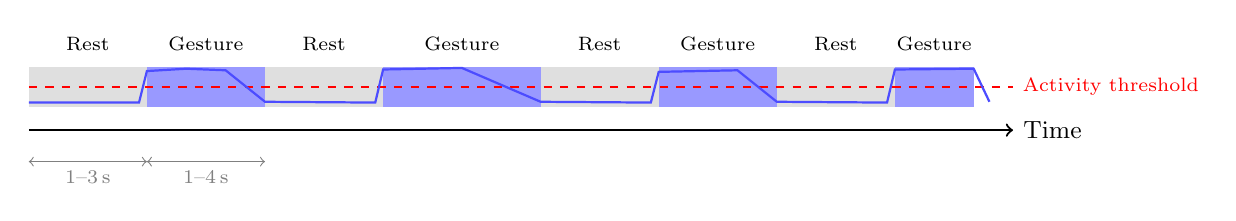
\begin{tikzpicture}[scale=1.0]
    \draw[thick, ->] (0,0) -- (12.5,0) node[right]{\small Time};

    \fill[gray!25] (0,0.3)    rectangle (1.5,0.8);
    \fill[gray!25] (3.0,0.3)  rectangle (4.5,0.8);
    \fill[gray!25] (6.5,0.3)  rectangle (8.0,0.8);
    \fill[gray!25] (9.5,0.3)  rectangle (11.0,0.8);

    \fill[blue!40] (1.5,0.3)  rectangle (3.0,0.8);
    \fill[blue!40] (4.5,0.3)  rectangle (6.5,0.8);
    \fill[blue!40] (8.0,0.3)  rectangle (9.5,0.8);
    \fill[blue!40] (11.0,0.3) rectangle (12.0,0.8);

    \node[font=\scriptsize] at (0.75, 1.1)  {Rest};
    \node[font=\scriptsize] at (2.25, 1.1)  {Gesture};
    \node[font=\scriptsize] at (3.75, 1.1)  {Rest};
    \node[font=\scriptsize] at (5.5,  1.1)  {Gesture};
    \node[font=\scriptsize] at (7.25, 1.1)  {Rest};
    \node[font=\scriptsize] at (8.75, 1.1)  {Gesture};
    \node[font=\scriptsize] at (10.25,1.1)  {Rest};
    \node[font=\scriptsize] at (11.5, 1.1)  {Gesture};

    \draw[<->, gray] (0,-0.4)   -- (1.5,-0.4)
        node[midway, below, font=\scriptsize]{1--3\,s};
    \draw[<->, gray] (1.5,-0.4) -- (3.0,-0.4)
        node[midway, below, font=\scriptsize]{1--4\,s};

    \draw[red, dashed, thick] (0,0.55) -- (12.5,0.55);
    \node[red, font=\scriptsize, right] at (12.5,0.55)
        {Activity threshold};

    \draw[blue!70, thick]
        (0,0.35)   -- (1.4,0.35) -- (1.5,0.75) -- (2.0,0.78)
        -- (2.5,0.76) -- (3.0,0.36) -- (4.4,0.35) -- (4.5,0.77)
        -- (5.5,0.79) -- (6.5,0.36) -- (7.9,0.35) -- (8.0,0.74)
        -- (9.0,0.76) -- (9.5,0.36) -- (10.9,0.35) -- (11.0,0.77)
        -- (12.0,0.78) -- (12.2,0.36);
\end{tikzpicture}
\caption{Schematic of the trial structure within a single EDF
recording. Active gesture periods (blue) alternate with rest
periods (gray). The activity gate threshold (red dashed line)
is used during preprocessing to retain only epochs where the
RMS energy exceeds the threshold, discarding rest-period epochs
that carry the gesture class label but contain no gesture signal.}
\label{fig:trial_structure}
\end{figure}

\subsection{Recording Files and Folder Organisation}

\begin{figure}[htbp]
\centering
\includegraphics[width=0.90\textwidth]{Assets/recording_software}
\caption{Screenshot of the EEG recording software showing live
multichannel EEG signals during a data collection session. All
19 channels are visible, with the characteristic large-amplitude
frontal deflections (Fp1, Fp2) clearly visible during blink
events.}
\label{fig:recording_software}
\end{figure}

Each recording session is organised into three sub-folders
corresponding to the three artifact modality groups:

\begin{itemize}[leftmargin=*]
    \item \textbf{Blink/} --- contains three \acrshort{edf} files,
    one for each blink type (BLINK01.edf for single blinks,
    BLINK02.edf for double blinks, BLINK03.edf for triple blinks).

    \item \textbf{Bruxissem/} --- contains two \acrshort{edf}
    files, one for left bruxism and one for right bruxism.
    Note: the folder name ``Bruxissem'' is retained from the
    original recording software output and is handled by the
    data loader.

    \item \textbf{Clinch/} --- contains \acrshort{edf} files
    for jaw clinch recordings. Clinch recordings were organised
    into sub-folders (Bilateral, Bileteral --- note the spelling
    variant, which was a typo in the folder naming that caused
    a silent data loss bug described in
    Section~\ref{sec:dc_bug}).
\end{itemize}

%% ----------------------------------------------------------
\section{Artifact Gesture Protocols}
\label{sec:dc_gestures}
%% ----------------------------------------------------------

This section provides detailed descriptions of each of the six
voluntary artifact gestures, including the physiological mechanism
by which each gesture produces a distinctive \acrshort{eeg}
signal, the recording instructions given to the subject, and
the characteristic signal morphology at the relevant electrode
sites.

\subsection{Single Blink (Class: \texttt{single\_blink})}

\textbf{Physiological mechanism:} A voluntary eye blink involves
a rapid closure and reopening of the eyelid driven by the
orbicularis oculi muscle, lasting approximately 150--400\,ms.
The movement of the eyelid over the cornea sweeps the
corneoretinal potential across the frontal scalp, inducing a
large-amplitude deflection primarily at Fp1 and Fp2. The signal
waveform is characterised by a single sharp negative or positive
peak (depending on the reference scheme) with amplitude
50--200\,\si{\micro\volt}, followed by a slower return to
baseline.

\textbf{Recording instruction:} The subject performed one
deliberate, complete eye blink, then waited 2--4\,seconds in a
relaxed eyes-open state before performing the next blink.
Approximately 60--80 single blinks were collected per session.

\textbf{Key electrodes:} Fp1, Fp2 (primary); F3, F4, F7, F8
(secondary, smaller amplitude).

\begin{figure}[htbp]
\centering

\includegraphics[width=0.90\textwidth]{Assets/signal_single_blink}
\caption{EEG signal at Fp1 and Fp2 during a voluntary single
blink. The characteristic single large-amplitude peak
(50--200\,\si{\micro\volt}) is clearly visible at both frontal
electrodes, with rapid onset and slower return to baseline.}
\label{fig:signal_single_blink}
\end{figure}

\subsection{Double Blink (Class: \texttt{double\_blink})}

\textbf{Physiological mechanism:} A double blink consists of
two complete blink cycles performed in rapid succession, with
an inter-blink interval of approximately 200--400\,ms. The
resulting \acrshort{eeg} signal at Fp1/Fp2 contains two
identifiable deflection peaks within a 600--900\,ms window,
distinguishing it from a single blink (one peak) and a triple
blink (three peaks).

\textbf{Recording instruction:} The subject performed two rapid
blinks in quick succession (``blink-blink''), then waited
3--5\,seconds before the next double blink. Approximately
50--70 double blinks were collected per session.

\textbf{Key electrodes:} Fp1, Fp2 (two peaks within window).

\textbf{Classification challenge:} The double blink is the
most difficult blink class to classify because its inter-blink
interval can vary, causing the second peak to sometimes fall
outside the 2\,s epoch window, making it appear as a single
blink. This is reflected in the lower F1 score (0.652) for
this class compared to single (0.885) and triple (0.721) blink.

\begin{figure}[htbp]
\centering

\includegraphics[width=0.90\textwidth]{Assets/signal_double_blink}
\caption{EEG signal at Fp1 and Fp2 during a voluntary double
blink. Two distinct amplitude peaks are visible within the 2\,s
epoch window, separated by an inter-blink interval of
approximately 200--400\,ms.}
\label{fig:signal_double_blink}
\end{figure}

\subsection{Triple Blink (Class: \texttt{triple\_blink})}

\textbf{Physiological mechanism:} A triple blink consists of
three complete blink cycles performed in rapid succession
(``blink-blink-blink''), with inter-blink intervals of
approximately 150--350\,ms each. The resulting signal contains
three identifiable peaks at Fp1/Fp2 within a 900--1{,}400\,ms
window.

\textbf{Recording instruction:} The subject performed three
rapid consecutive blinks, then waited 4--6\,seconds before the
next triple blink. Approximately 40--60 triple blinks were
collected per session.

\textbf{Key electrodes:} Fp1, Fp2 (three peaks within window).

\textbf{Classification challenge:} Triple blinks tend to
confuse with double blinks at the boundary: if the subject
performs a triple blink slightly more slowly than usual, the
third blink may fall outside the epoch window, making the epoch
appear as a double blink. The S~$\leftrightarrow$~T confusion
pair in the confusion matrix (Chapter~8) reflects this overlap.

\begin{figure}[htbp]
\centering

\includegraphics[width=0.90\textwidth]{Assets/signal_triple_blink}
\caption{EEG signal at Fp1 and Fp2 during a voluntary triple
blink. Three distinct amplitude peaks are visible within the
2\,s window. The third peak is sometimes truncated when the
inter-blink interval is slightly longer than average,
contributing to S$\leftrightarrow$T confusion.}
\label{fig:signal_triple_blink}
\end{figure}

\subsection{Jaw Clinch (Class: \texttt{clinch})}

\textbf{Physiological mechanism:} A jaw clinch involves a
sustained, forceful bilateral contraction of the masseter and
temporalis muscles, as in biting down hard. The muscle
contraction produces a broadband \acrshort{emg} burst
(30--200\,Hz) that contaminates both temporal channels (T3, T4)
simultaneously with high-amplitude signals (often
$>$100\,\si{\micro\volt} at the electrode after broadband
filtering). The bilateral symmetry of the clinch --- roughly
equal activation of T3 and T4 --- distinguishes it from bruxism.

\textbf{Recording instruction:} The subject performed a firm
jaw clinch lasting approximately 1--2\,seconds, then relaxed
and waited 3--4\,seconds before the next clinch. This is the
highest-epoch-count class in the dataset (1{,}328 epochs) due
to the ease and comfort of performing sustained clinches.

\textbf{Key electrodes:} T3 and T4 (bilateral, approximately
equal amplitude); T5, T6 (secondary).

\textbf{Loader bug and its impact:} Section~\ref{sec:dc_bug}
describes a critical data loader bug that caused 25\% of clinch
data (326 epochs) to be silently discarded during initial
training runs, due to a folder naming typo.

\begin{figure}[htbp]
\centering

\includegraphics[width=0.90\textwidth]{Assets/signal_clinch}
\caption{EEG signal at T3 and T4 during a voluntary jaw clinch.
Both temporal channels show simultaneous large-amplitude
broadband EMG bursts with approximately equal amplitude
(bilateral symmetry), clearly distinguishable from the resting
baseline before and after the clinch.}
\label{fig:signal_clinch}
\end{figure}

\subsection{Left Bruxism (Class: \texttt{bruxism\_left})}

\textbf{Physiological mechanism:} Bruxism refers to lateral jaw
grinding movements. Left bruxism involves grinding the lower jaw
to the left side relative to the upper jaw, producing preferential
activation of the left temporalis muscle. This lateralised
contraction is captured as a higher-amplitude \acrshort{emg}
signal at T3 (left temporal) compared to T4 (right temporal).

\textbf{Recording instruction:} The subject performed a
deliberate left-directed grinding motion lasting approximately
1\,second, then relaxed and waited 3--5\,seconds before the
next repetition. The subject was instructed to make the motion
feel distinct from a simple clinch by emphasising the leftward
jaw displacement.

\textbf{Key electrodes:} T3 $>$ T4 (T3 dominant); normalised
asymmetry index $(T4 - T3)/(T4 + T3) < 0$.

\begin{figure}[htbp]
\centering

\includegraphics[width=0.90\textwidth]{Assets/signal_bruxism_l}
\caption{EEG signal at T3 and T4 during voluntary \textbf{left
bruxism}. T3 (left temporal) shows clearly higher amplitude
than T4 (right temporal), reflecting preferential activation
of the left temporalis muscle. The normalised asymmetry index
$\mathcal{A}_{T3,T4} < 0$ for this class.}
\label{fig:signal_bruxism_left}
\end{figure}

\subsection{Right Bruxism (Class: \texttt{bruxism\_right})}

\textbf{Physiological mechanism:} Right bruxism involves
grinding the lower jaw to the right side, producing preferential
activation of the right temporalis muscle, captured as a
higher-amplitude signal at T4 (right temporal) compared to T3.

\textbf{Recording instruction:} The subject performed a
deliberate right-directed grinding motion lasting approximately
1\,second, then relaxed and waited 3--5\,seconds before the
next repetition.

\textbf{Key electrodes:} T4 $>$ T3 (T4 dominant); normalised
asymmetry index $(T4 - T3)/(T4 + T3) > 0$.

\begin{figure}[htbp]
\centering

\includegraphics[width=0.90\textwidth]{Assets/signal_bruxism_r}
\caption{EEG signal at T3 and T4 during voluntary \textbf{right
bruxism}. T4 (right temporal) shows clearly higher amplitude
than T3 (left temporal), reflecting preferential activation
of the right temporalis muscle. The normalised asymmetry index
$\mathcal{A}_{T3,T4} > 0$ for this class. Comparing this
figure with Figure~\ref{fig:signal_bruxism_left} clearly
demonstrates the lateral asymmetry that the T3--T4 asymmetry
index (Chapter~6) is designed to capture.}
\label{fig:signal_bruxism_right}
\end{figure}

%% ----------------------------------------------------------
\section{Data Directory Structure}
\label{sec:dc_structure}
%% ----------------------------------------------------------

The complete dataset is organised in a hierarchical directory
structure that the data loader (\code{loader.py}) traverses
automatically. The structure is as follows:

\begin{lstlisting}[language=bash, caption={Dataset directory
structure. Each Session directory contains three sub-folders
corresponding to the three artifact modality groups. Each EDF
file contains one continuous recording of a single artifact
class.}, label={lst:dir_structure}]
DATA/
|-- Session1/               # Training data - Session 1
|   |-- Blink/
|   |   |-- BLINK01.edf    # Single blink recordings
|   |   |-- BLINK02.edf    # Double blink recordings
|   |   `-- BLINK03.edf    # Triple blink recordings
|   |-- Bruxissem/
|   |   |-- LEFT.edf       # Left bruxism recordings
|   |   `-- RIGHT.edf      # Right bruxism recordings
|   `-- Clinch/
|       |-- Bilateral/
|       |   `-- *.edf      # Bilateral clinch recordings
|       `-- Bileteral/     # Typo variant - also loaded
|           `-- *.edf
|-- Session2/               # Training data - Session 2
|   |-- Blink/             # Same structure as Session1
|   |-- Bruxissem/
|   `-- Clinch/
|-- Session3/               # Training data - incoming
|   `-- (same structure)
|-- Dev/                    # Held-out development set
|   `-- *.edf + markers.csv
`-- Test/                   # Held-out test set (untouched)
    `-- *.edf + markers.csv
\end{lstlisting}

\subsection{Loader Design and Auto-Scanning}

The data loader (\code{loader.py}) was designed to automatically
discover and load all \acrshort{edf} files matching the expected
class patterns, without requiring manual file path specification.
The loader performs the following steps:

\begin{enumerate}[leftmargin=*]
    \item Scan the \code{DATA/} root directory for all
    sub-directories matching the pattern \code{Session*}.
    \item Within each session directory, search for
    \code{Blink/}, \code{Bruxissem/}, and \code{Clinch/}
    sub-directories.
    \item Within \code{Blink/}, match files named
    \code{BLINK01.edf}, \code{BLINK02.edf}, \code{BLINK03.edf}
    and assign labels \code{single\_blink}, \code{double\_blink},
    \code{triple\_blink} respectively.
    \item Within \code{Bruxissem/}, match files containing
    \code{LEFT} or \code{RIGHT} in their filename.
    \item Within \code{Clinch/}, recursively search all
    sub-directories for \acrshort{edf} files and assign the
    \code{clinch} label. This recursive search handles all
    spelling variants of the \code{Bilateral}/\code{Bileteral}
    sub-folder name.
    \item Return a list of \code{(filepath, label)} tuples
    covering all discovered files across all sessions.
\end{enumerate}

In the current dataset (Session1 + Session2), the loader
successfully discovers and loads all 18 \acrshort{edf} files.

\subsection{Loader Bug: Silent Clinch Data Loss}
\label{sec:dc_bug}

During initial development, a critical bug was discovered in
the data loader that caused approximately 25\% of clinch training
data to be silently discarded. The root cause was a folder naming
inconsistency: the recording software saved clinch recordings
from one sub-session into a folder named \textbf{``Bileteral''}
(a typographical error) rather than the expected
\textbf{``Bilateral''}. The original loader recognised only
``Bilateral'' and ``Both'' as valid folder names, causing the
typo variant to be silently skipped.

\textbf{Impact:} The loader was processing only 1{,}002 clinch
epochs instead of the correct 1{,}328 --- a reduction of 326
epochs (24.6\%). Since clinch is the highest-performing class
(F1 = 0.916), the impact on overall accuracy was limited, but
the silent nature of the failure is concerning: the system gave
no warning that data was being dropped, making the bug difficult
to diagnose.

\textbf{Fix:} The loader was updated to perform
case-insensitive recursive scanning of all sub-directories under
\code{Clinch/}, accepting any folder name. A validation report
is now printed on startup listing the number of \acrshort{edf}
files discovered per class, enabling quick visual verification
that no files are being missed.

%% ----------------------------------------------------------
\section{Dataset Statistics}
\label{sec:dc_stats}
%% ----------------------------------------------------------

\subsection{Raw Epoch Counts}

After applying the complete preprocessing and activity gating
pipeline (described in Chapters~5 and~6), the final dataset
used for training and evaluation contains the epoch counts
shown in Table~\ref{tab:dataset_stats}.

\begin{table}[htbp]
\centering
\caption{Dataset statistics after activity-gated epoch
extraction. Epochs are pooled across Session1 and Session2.
The ``Before Gating'' column shows the total epoch count
including rest windows; ``After Gating'' shows the count
after applying the RMS activity threshold.}
\label{tab:dataset_stats}
\renewcommand{\arraystretch}{1.3}
\begin{tabular}{l c c c c}
\toprule
\textbf{Class} & \textbf{Label} &
\textbf{Before Gate} & \textbf{After Gate} &
\textbf{Retained (\%)} \\
\midrule
Single blink  & \code{single\_blink}  & 812     & 390     & 48.0\% \\
Double blink  & \code{double\_blink}  & 702     & 337     & 48.0\% \\
Triple blink  & \code{triple\_blink}  & 575     & 276     & 48.0\% \\
Jaw clinch    & \code{clinch}         & 2{,}767 & 1{,}328 & 48.0\% \\
Bruxism left  & \code{bruxism\_left}  & 450     & 216     & 48.0\% \\
Bruxism right & \code{bruxism\_right} & 571     & 274     & 48.0\% \\
\midrule
\textbf{Total} & & \textbf{5{,}877} & \textbf{2{,}821} &
\textbf{48.0\%} \\
\bottomrule
\end{tabular}
\end{table}

The consistent 48\% retention rate across all classes confirms
that the activity gate is behaving as expected: approximately
half of each recording consists of rest windows (the subject
pausing between gestures), and the gate correctly identifies
and removes these windows regardless of the artifact class.

\subsection{Class Imbalance}

Figure~\ref{fig:class_distribution} illustrates the class
distribution after activity gating. The dataset exhibits
moderate class imbalance, with clinch (1{,}328 epochs) being
approximately 6$\times$ more frequent than bruxism\_left
(216 epochs). This imbalance arises from two sources: (1) the
relative ease of sustaining a clinch gesture, which produces
longer continuous active windows; and (2) the higher inherent
variability of bruxism gestures, which leads to more epochs
being rejected by the activity gate due to insufficient energy.

\begin{figure}[htbp]
\centering
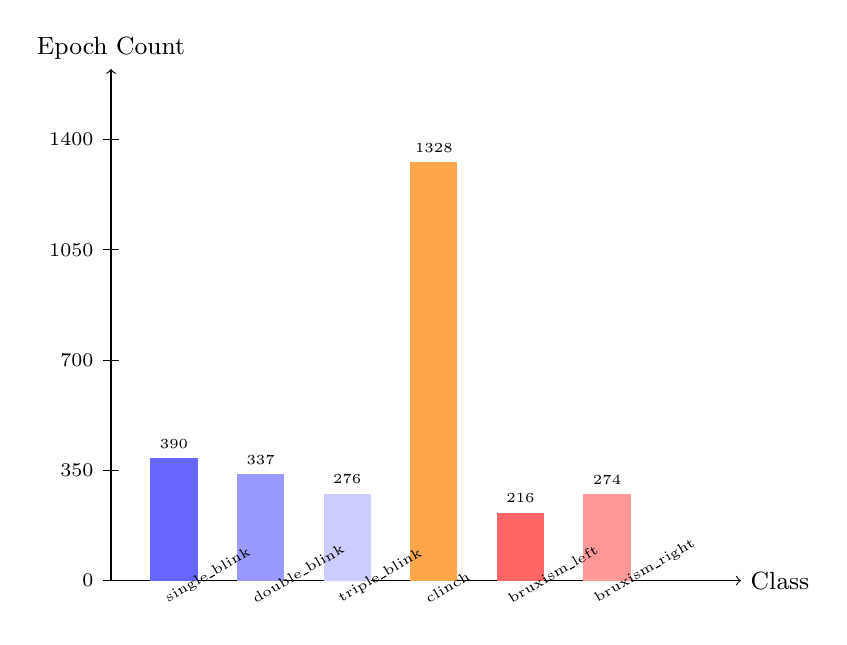
\begin{tikzpicture}
\begin{scope}
    \draw[->] (0,0) -- (8,0) node[right]{\small Class};
    \draw[->] (0,0) -- (0,6.5) node[above]{\small Epoch Count};

    \foreach \y/\label in {0/0, 1.4/350, 2.8/700,
                            4.2/1050, 5.6/1400}{
        \draw (-0.1,\y) -- (0.1,\y);
        \node[left, font=\scriptsize] at (-0.1,\y) {\label};
    }

    \fill[blue!60]   (0.5,0) rectangle (1.1, 1.56);
    \node[font=\tiny, above] at (0.8,  1.56)  {390};
    \fill[blue!40]   (1.6,0) rectangle (2.2, 1.348);
    \node[font=\tiny, above] at (1.9,  1.348) {337};
    \fill[blue!20]   (2.7,0) rectangle (3.3, 1.104);
    \node[font=\tiny, above] at (3.0,  1.104) {276};
    \fill[orange!70] (3.8,0) rectangle (4.4, 5.312);
    \node[font=\tiny, above] at (4.1,  5.312) {1328};
    \fill[red!60]    (4.9,0) rectangle (5.5, 0.864);
    \node[font=\tiny, above] at (5.2,  0.864) {216};
    \fill[red!40]    (6.0,0) rectangle (6.6, 1.096);
    \node[font=\tiny, above] at (6.3,  1.096) {274};

    \node[font=\tiny, rotate=30, anchor=west] at (0.6,-0.3)
        {single\_blink};
    \node[font=\tiny, rotate=30, anchor=west] at (1.7,-0.3)
        {double\_blink};
    \node[font=\tiny, rotate=30, anchor=west] at (2.8,-0.3)
        {triple\_blink};
    \node[font=\tiny, rotate=30, anchor=west] at (3.9,-0.3)
        {clinch};
    \node[font=\tiny, rotate=30, anchor=west] at (4.95,-0.3)
        {bruxism\_left};
    \node[font=\tiny, rotate=30, anchor=west] at (6.05,-0.3)
        {bruxism\_right};
\end{scope}
\end{tikzpicture}
\caption{Class distribution of the final activity-gated dataset
(2{,}821 epochs total). Clinch is the dominant class (1{,}328
epochs) due to the ease of sustained clinch gestures. Bruxism
classes have the lowest epoch counts (216--274 epochs). Class
imbalance is addressed during training using SMOTE (Chapter~7).}
\label{fig:class_distribution}
\end{figure}

\subsection{Session-Level Statistics}

Table~\ref{tab:session_stats} breaks down the epoch counts by
session, confirming that both sessions contribute meaningfully
to all six classes.

\begin{table}[htbp]
\centering
\caption{Epoch counts per class per session after activity
gating. Session3 data will be added upon completion.}
\label{tab:session_stats}
\renewcommand{\arraystretch}{1.3}
\begin{tabular}{l c c c}
\toprule
\textbf{Class} & \textbf{Session1} & \textbf{Session2} &
\textbf{Total} \\
\midrule
single\_blink  & $\approx$195 & $\approx$195 & 390 \\
double\_blink  & $\approx$169 & $\approx$168 & 337 \\
triple\_blink  & $\approx$138 & $\approx$138 & 276 \\
clinch         & $\approx$664 & $\approx$664 & 1{,}328 \\
bruxism\_left  & $\approx$108 & $\approx$108 & 216 \\
bruxism\_right & $\approx$137 & $\approx$137 & 274 \\
\midrule
\textbf{Total} & $\approx$1{,}411 & $\approx$1{,}410 &
\textbf{2{,}821} \\
\bottomrule
\end{tabular}
\end{table}

%% ----------------------------------------------------------
\section{Label Scheme Evolution: 5 Classes to 6 Classes}
\label{sec:dc_labels}
%% ----------------------------------------------------------

An important design decision made during the data collection
and labelling phase concerns the blink class structure. In the
initial version of the system, single blinks (BLINK01) and
multiple blinks were merged into a single class, based on the
assumption that they could be treated as a single ``blink''
command. This produced a 5-class label scheme:
\{single/triple blink, double blink, clinch, bruxism\_left,
bruxism\_right\}.

This merging decision proved to be a significant error.
BLINK01 recordings contain single blinks, while BLINK03
recordings contain triple blinks. A recording session of single
blinks (BLINK01) contains long rest periods between sparse
single blink events, while a session of triple blinks (BLINK03)
contains longer active windows with three closely spaced peaks.
When these two recordings were merged into one class, the
training data for that class contained contradictory examples:
some epochs showed a single peak (from BLINK01 rest periods
with a single blink at the edge), others showed three peaks
(from BLINK03 active windows). The classifier could not learn
a consistent decision boundary for this class.

The fix was to separate all three blink types into three
independent classes --- \code{single\_blink},
\code{double\_blink}, and \code{triple\_blink} --- each sourced
exclusively from the corresponding recording file. This produced
a 6-class scheme with pure, unambiguous training examples for
each blink type.

\textbf{Quantitative impact:} The 5~$\rightarrow$~6 class
change improved overall accuracy from 80.4\% to 83.4\%
(+3.0\%), with the largest improvements in the blink and
bruxism classes that were most affected by the contaminated
training data:

\begin{itemize}[leftmargin=*]
    \item single\_blink F1: $0.818 \rightarrow 0.885$ (+0.067)
    \item bruxism\_left F1: $0.609 \rightarrow 0.737$ (+0.128)
    \item bruxism\_right F1: $0.686 \rightarrow 0.755$ (+0.069)
\end{itemize}

%% ----------------------------------------------------------
\section{Development and Test Set Design}
\label{sec:dc_devtest}
%% ----------------------------------------------------------

In addition to the training sessions (Session1 and Session2),
two held-out evaluation sets were designed for system validation:

\textbf{Development set (Dev/):} A 10-minute \acrshort{eeg}
recording in a free-running, mixed-gesture paradigm --- the
subject performs gestures in any order at will, without
separating gestures by class into separate files. An
accompanying CSV file (\code{markers.csv}) records the timestamp
and class label of each gesture as it is performed, enabling
precise epoch extraction aligned to actual gesture events. The
development set is used for hyperparameter tuning and threshold
calibration (\code{ACTIVITY\_THRESHOLD}, \code{CONF\_THRESH},
\code{FSM\_THRESH}) without touching the test set.

\textbf{Test set (Test/):} A second 10-minute mixed-gesture
recording with an accompanying \code{markers.csv}, held
completely untouched until final system evaluation. The test
set is used only once --- for the final accuracy report
submitted with this project. No design decisions, threshold
adjustments, or model changes are made after the test set is
first evaluated.

This train/dev/test split methodology follows best practices
in machine learning~\cite{pedregosa2011sklearn} and ensures
that the reported test accuracy is a genuine estimate of
real-world performance, not an optimistic artefact of repeated
evaluation on the same data. At the time of writing, both the
Dev and Test sets are scheduled to be recorded following the
completion of Session3.

%% ----------------------------------------------------------
\section{Chapter Summary}
\label{sec:dc_summary}
%% ----------------------------------------------------------

This chapter described the complete data collection methodology
for the \acrshort{bci} dataset. A single subject performed six
classes of voluntary \acrshort{eeg} artifact gestures --- single
blink, double blink, triple blink, jaw clinch, left bruxism,
and right bruxism --- across two independent recording sessions
(Session1 and Session2), producing 18 \acrshort{edf} files
organised in a hierarchical directory structure. After
activity-gated epoch extraction (described in Chapter~5), the
dataset contains 2{,}821 epochs across the six classes. A
critical data loader bug that silently discarded 326 clinch
epochs (24.6\%) was identified and corrected. A label scheme
evolution from 5 to 6 classes (+3.0\% accuracy) was described.
Held-out development and test sets with marker-aligned CSV
annotations are planned for final system evaluation. The
following chapter describes in detail the signal processing
pipeline applied to the raw \acrshort{edf} recordings.